
\documentclass[12pt]{article}
\usepackage[margin=1in]{geometry}
\usepackage{setspace}
\usepackage{float}
\usepackage{graphicx}
\graphicspath{{images/}}

\title{Determining the Overhead of the EZTrace System}
\author{Philip M. Westrich}
\date{May 1, 2017}

\begin{document}

\maketitle
\vspace{-0.3in}\noindent\rule{\linewidth}{0.4pt}
\doublespacing

\begin{abstract}

    High performance computing plays an integral role in modern science. Many will use large scale simulations to test 
    things from new theories in astrophysics to determining the next week's weather. These simulations depend on the 
    programs written to carry them out; if they are incorrect or inefficient, they may possibly hinder their progress 
    rather than help it.
    
    The people who run these simulations always would like to make them faster; no one likes long wait times. Two methods 
    used to determine the inefficiencies in large parallel or distributed systems are tracing and logging. However, they 
    both do not come for free. On the extreme end, parallel debuggers can slow down a program up to 1000 times!
    
    In this paper, we will test the tracing system EZTrace and determine how much of a performance penalty it introduces 
    into a system.\\
 
\end{abstract}

\vspace{-0.3in}\noindent\rule{\linewidth}{0.4pt}
\pagebreak

\section{Introduction}

Large scale simulations are used all over the place to model hard to test phenomenon in modern science. As these models 
become more complex and the simulations used to predict according to them become more and more complex, they require more 
computational power, time, or both to produce accurate enough results.

In order to prevent resources from being wasted, it is important that the algorithms used are as efficient as possible. 
The difference between $ O(n^{2.5}) $ and $ O(n^3) $ in computation or communication could mean hundreds of hours per 
simulation wasted.

\subsection{Tracing and profiling}

Two related methods used to discern the reasons behind poor performance are tracing and profiling. They have been used 
for decades to discern the reasons a program is either producing incorrect results or operating inefficiently.

Program tracing is the process of annotating a program with code such that it records the sequence of defined blocks a 
program executes, and running the modified program to collect this data into a trace file. Program profiling counts the 
number of times those defined blocks are executed in a program's lifetime. \cite{Ball1994, Larus1993} 

However, tracing and profiling do not come for free. Since they usually involve inserting extra code into a program to 
execute, there is naturally some nonzero amount of overhead introduced that increases as the number of blocks to measure 
increases. The data generated from the process can and oftentimes quickly grows to such a size that it either physically 
cannot be stored on available storage, or it becomes impractical to sort through for any meaning. Therefore, it is 
imperative that the systems that perform the tracing or profiling are as efficient as possible with both time and storage 
space. \cite{Ball1994, Larus1993, Mohror2012}

Tools have been written that can do tracing and profiling in a decently efficient manner, but there are still some limitations 
to what they can do. In the parallel computing world, there are numerous tools that can profile standard libraries, such as 
OpenMP, MPI, POSIX threads, and others. However, when it comes to instrumenting user-defined functions, those tools fall 
short, and the developer must resort to manual instrumentation. They also do not allow for different interpretation of 
events; once an even is written, some data is lost and there is no other way to interpret it. \cite{Trahay2011} 

\subsection{The EZTrace system}

These complex systems require complicated tools to analyze them, especially once parallel and distributed computing are 
introduced. One solution presented was the EZTrace performance analysis framework. The authors of the framework state 
that they have written EZTrace with the aforementioned issues in mind. \cite{Trahay2011}

The EZTrace system is plugin-based. It comes with several preinstalled plugins for analysis of the common parallel and 
distributed programming libraries: OpenMP, MPI, POSIX threads, and the PLASMA library. It also gives a method for a 
developer to define their own to handle other code in their program. This way, most parellel systems can be automatically 
analyzed with minimal effort from the developer, but if they decide more is needed, they can write a plugin. \cite{Trahay2011}

The EZTrace system has a two-phase system. In the first, while the program is running, events are recorded. In the second, 
after the program is finished, these events are then interpreted. This allows for decoupled recording and interpretation; 
the user can treat an event in whichever way they wish depending on other context. It also means that more expensive 
operations can be placed in the second phase, while the first focuses only on data retention. \cite{Trahay2011}

In their paper, the authors claim that the EZTrace system performs all the aforementioned tasks in an efficient manner. 
In this paper, we intend to duplicate their results.

\section{Testing methods}

In their paper, the authors of the EZTrace system used the NAS Parallel Benchmark suite \cite{Bailey1991} to show that the 
overhead their system introduced was indeed minimal compared to other tracing systems. For this paper, we ran the same 
benchmarks at the same sizes and number of threads as they did. Since the resources were available, we ran them at a 
larger size as well. \cite{Trahay2011}

The partition of the high performance cluster that was used consists of four nodes, each with dual Intel Xeon E5-2680v4 
and 128 GB of RAM, and was running Debian 7.10. Each benchmark ran was submitted to the batch queuing system and was 
restricted to those nodes. Each test was run on a single node by itself.

The latest version of the benchmarks at the time of writing this paper (3.3.1) were downloaded and compiled on the compute 
nodes for size classes B, C, and D, except for the FT benchmark, which could not be compiled for size D. While the university 
has the resources to also execute size class E, it could not be done because the cluster was not free enough to accommodate 
them, and the jobs would not have finished fast enough in time to write this paper.

Benchmarks that required a perfect square number of processes were built for 36 processes, and all others were built for 
32. EZTrace was installed from the Debian repository, which gave version 0.7-2-4. EZTrace was told to trace the MPI calls 
from each benchmark. Due to time constraints, each benchmark was executed once with EZTrace and once without.

\section{Results}

The results from the tests are in the following tables. 

\begin{table}[H]
\centering
\caption{Execution time (s), without EZTrace}
\label{tab:notrace}
\begin{tabular}{|l|cccccccc|}
\hline
Class & BT      & CG     & EP     & FT   & IS    & LU      & MG     & SP      \\ \hline
B     & 22.07   & 5.28   & 3.04   & 5.46 & 0.45  & 14.54   & 1.36   & 26.42   \\
C     & 91.72   & 19.87  & 10.53  & 21.8 & 1.61  & 56.25   & 7.33   & 104.88  \\
D     & 1655.87 & 710.35 & 146.11 &      & 25.33 & 1330.85 & 170.91 & 2046.87 \\
\hline
\end{tabular}
\end{table}

\begin{table}[H]
\centering
\caption{Execution time (s), with EZTrace}
\label{tab:eztrace}
\begin{tabular}{|l|cccccccc|}
\hline
Class & BT      & CG     & EP     & FT    & IS    & LU      & MG     & SP      \\ \hline
B     & 21.88   & 7.19   & 3.08   & 5.53  & 0.53  & 15.25   & 1.38   & 23.40   \\
C     & 89.27   & 18.43  & 10.07  & 20.28 & 1.80  & 66.12   & 8.39   & 106.32  \\
D     & 1654.77 & 779.60 & 147.66 &       & 27.79 & 1320.66 & 172.21 & 2207.90 \\
\hline
\end{tabular}
\end{table}

\begin{table}[H]
\centering
\caption{EZTrace overhead}
\label{tab:overhead}
\begin{tabular}{|l|cccccccc|}
\hline
Class & BT      & CG      & EP      & FT      & IS      & LU      & MG      & SP       \\ \hline
B     & -0.86\% & 36.17\% & 1.32\%  & 1.28\%  & 17.78\% & 4.88\%  & 1.47\%  & -11.43\% \\
C     & -2.67\% & -7.25\% & -4.37\% & -4.25\% & 11.80\% & 17.55\% & 14.46\% & 1.37\%   \\
D     & -0.07\% & 9.75\%  & 1.06\%  &         & 9.71\%  & -0.77\% & 0.76\%  & 7.87\%   \\
\hline
\end{tabular}
\end{table}

\begin{figure}[H]
\caption{The results from the previous paper \cite{Trahay2011}}
\label{fig:previous}
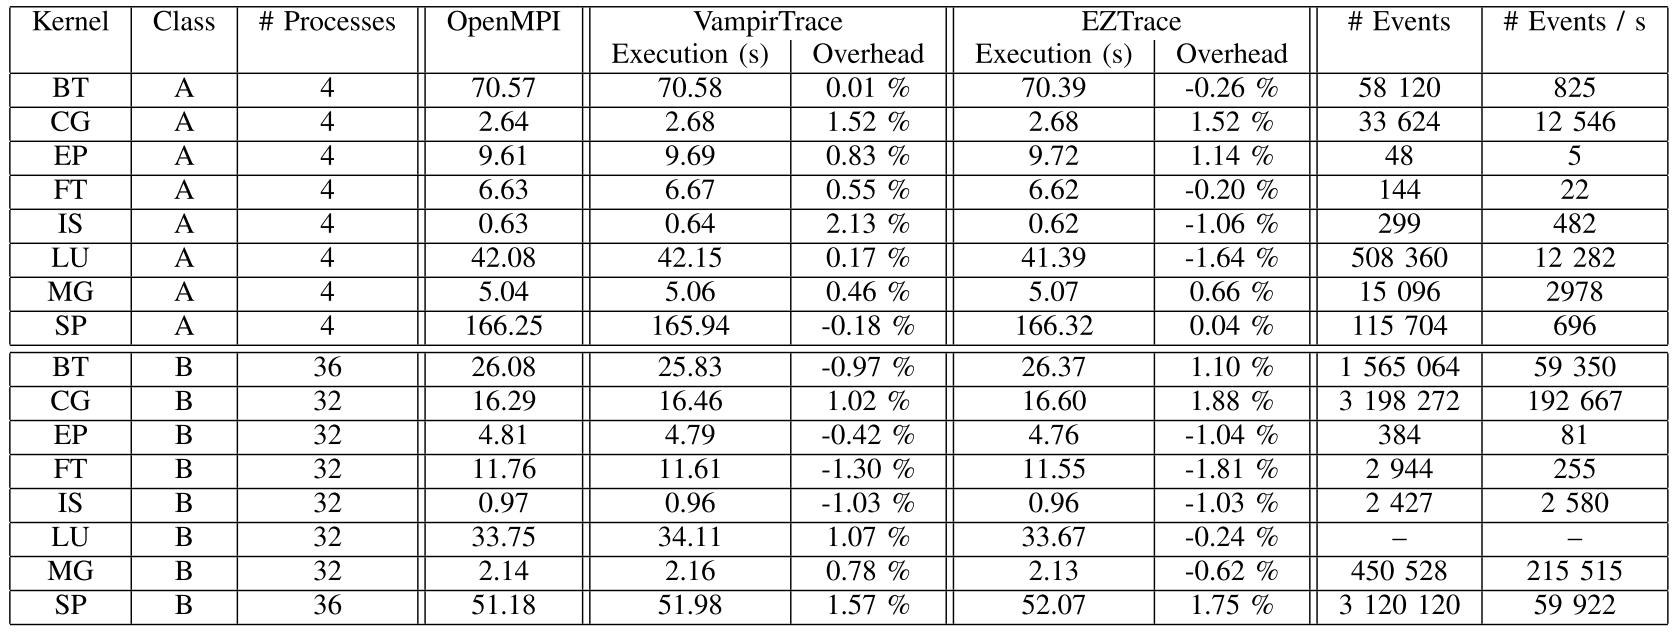
\includegraphics[scale=0.6]{eztrace_results}
\centering
\end{figure}

\begin{figure}[H]
\caption{Overhead as the size class increases}
\label{fig:overhead}
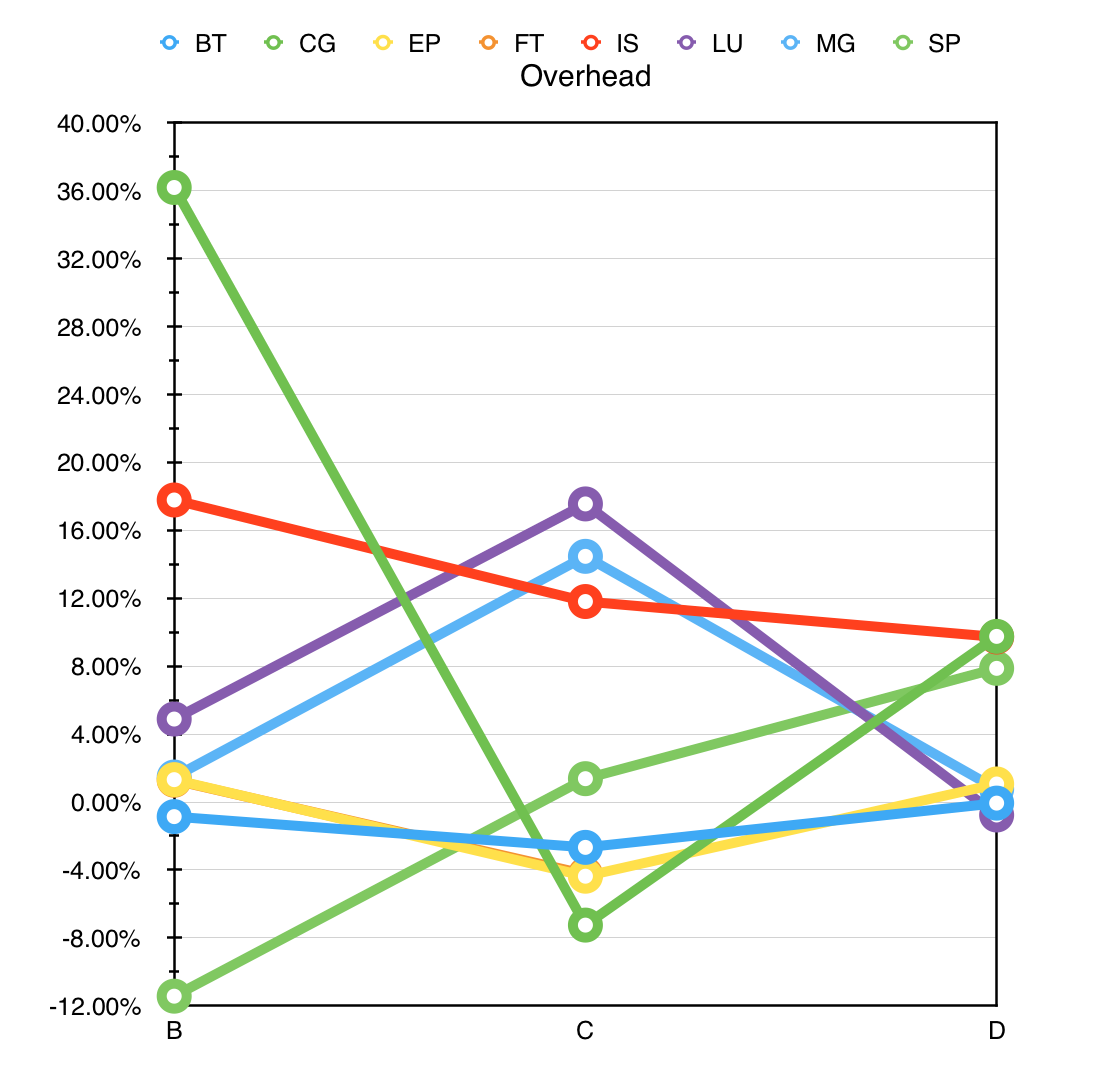
\includegraphics[scale=0.5]{overhead_graphs}
\centering
\end{figure}

\subsection{Discussion}

As can be seen from Figure~\ref{fig:overhead}, there is no clear-cut trend in the amount of overhead as the problem size 
increases. In some cases, EZTrace took noticeably longer, such as with CG class B or LU class C. However, in other benchmarks, 
the EZTrace benchmarks were faster, such as in SP class B. 

This does mirror slightly the results that the authors of EZTrace got in their tests in Figure~\ref{fig:previous} \cite{Trahay2011}. 
We had hoped that a trend would have been more defined when running the benchmarks for larger size classes, but that was 
not the case.

\subsection{Possible improvements}

Since the tests we performed were not very conclusive, there is obviously some room for improvement. Most notably, the 
benchmarks need to be run more times than just once. An average of those times would help remove some of the other factors 
that affect a program's runtime, such as other processes running on the machine and what the operating system decides to 
do with them.

It also would have been interesting to see how running the benchmarks across multiple nodes would have affected the overhead 
measurements. Since many MPI programs tend to spend plenty of time waiting for messages to be passed, it is possible that 
the time spend in communication could have outweighed EZTrace's computation enough that it did not appear. In programs of 
that nature, running EZTrace would not be noticeable. It would have also reflected the EZTrace system's authors test setup 
better.

One performance bottleneck in our test setup is the disk I/O speed. The home folders for user accounts are mapped to a 
central shared network drive. While this is very convenient for the users of the system in the fact that all of their 
files are in the exact same location regardless of the machine they log on to, it is noticeably slow. Many systems across 
the university with many users logged on are all accessing this shared storage at once. Therefore, our benchmarks may end 
up spending lots of time idling when writing to disk, and that time is nondeterministic depending on what other users on 
the university are doing at that give time. For testing purposes, it would be ideal to remove this variable.

\section{Conclusion}

In this paper, we ran the NAS Parallel Benchmark suite \cite{Bailey1991} on the university's high performance computing 
cluster in order to determine the overhead that the EZTrace automatic paralell program tracing framework \cite{Trahay2011} 
adds to a system. 

However, the results from our test were not very conclusive. The overhead amounts did not appear to set any clear trend. 
More testing is needed to determine the efficiency of the framework. This mirrors the results that the authors of EZTrace 
got in their tests. \cite{Trahay2011}. 

\bibliographystyle{acm}
\bibliography{bibliography.bib}

\end{document}
